\documentclass[main.tex]{subfiles}

\begin{document}

\section{Coding and Integration}

After a brief overview of the project and the project plan, this section will focus on the main technologies used in the project and the rationale behind choosing them. Moving on, we will discuss how these components were integrated and eventually deployed.

\subsection{Overview}

One of the first decisions made this term was to completely recreate our prototype of Thalia. This radical move was the consequence of a new implementation decision (for more detail see \ref{Web Framework}) and designed to give us the opportunity to refine the structure and quality of our code. The team determined this decision to be reasonable, as prototypes are meant to be disposable and are designed only to answer key questions about the system \cite{pragmaticprog}.

Despite the risks posed by the use of a Software Version Control (SVC) host such as GitHub, we have decided to continue using it as our software development platform. The reasoning behind this builds on the argument developed in last semester's Technical Report \cite{TR}, which highlights that our Data Processing Module is a separate component of our system that none of the other components are able to access. Additionally, we are storing API keys as environment variables in a file that is not tracked by our SVC system, which minimizes the risk of accidental exposure of sensitive data.

We have also decided to develop the application with Python as our main choice of programming language. Even though this choice seemed obvious from the beginning, we did consider its main benefits, which are as follows:

\begin{itemize}
    \item Python is a high level programming language allowing us to focus on the application.
    \item A standard choice for prototyping.
    \item Provides superb third-party libraries and frameworks free of charge.
    \item Easy to integrate with other languages if we were to choose to do so at a later stage of development.
    \item The whole team was already familiar with the language, saving us the precious time needed to learn another programming language.
    \item Our application does not require an unreasonable amount of computation, so there is no need for a more efficient programming language such as C \ref{BL} \cite{languagescomparison}.
\end{itemize}

We will discuss other technologies used in more detail after the discussion on project planning.

\subsection{Planning}

%Egalitarian team structure capitalization is wierd, wouldnt it be an egalitaion team structure or the Ega. Tea. Structure 'model/method/...'
Early in the inception phase of development, we decided to adopt the Egalitarian Team structure to make use of the flexibility offered by it. This meant that individual team members would not have fixed responsibilities, allowing anybody to work on each of the systems components. This decision also eased the code review process, as there were no internal power dynamics that might have adversely affected the error-correcting mechanism \cite{statusdifference}. Furthermore, since no team member was the sole developer of a system component, this meant review comments could be directed at the code and not an individual author \cite{howtoreview}. 

Our workflow was centred around the tools provided by GitHub. We used a ticketing system to divide and distribute tasks among team members. These tickets were usually allocated by the team at the weekly meetings, but occasionally they were chosen by the person proposing the feature or change. Our goal with this approach was to divide larger jobs into smaller tasks, so units of work could be completed in a single sprint in line with our Agile development approach.

A typical ticket in our project was an encapsulation of a user story, which consisted of a title, a one line description, value, acceptance criteria, and subtasks. In the first half of development, we also used effort-oriented metrics (story points) to measure the amount of work incurred by taking on a ticket, but, as previously mentioned, we later decided to abandon this aspect. An example of a ticket can be seen on \figurename{\ref{Ticket}}.

\begin{figure}[H]
   \centering
   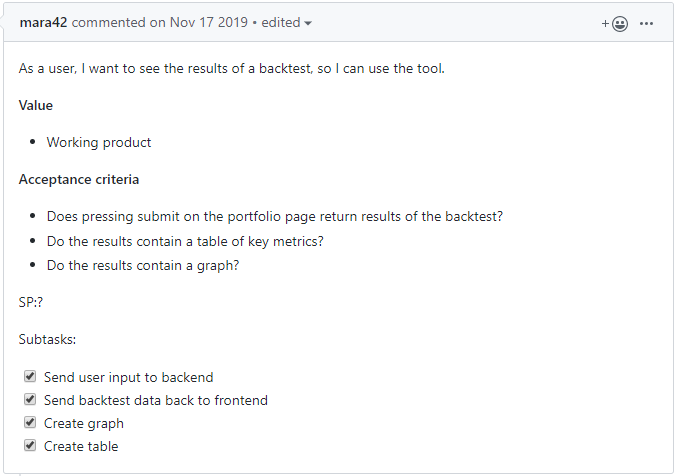
\includegraphics[scale=0.7]{05Coding/05Pictures/ticket.png}
   \caption{Ticket Example (source: https://github.com/)}
   \label{Ticket}
\end{figure}

Throughout the whole project, we had a total of 110 tickets and 71 pull requests. The following graph also shows the number of contributions to the master branch, excluding merge commits.

\begin{figure}[H]
   \centering
   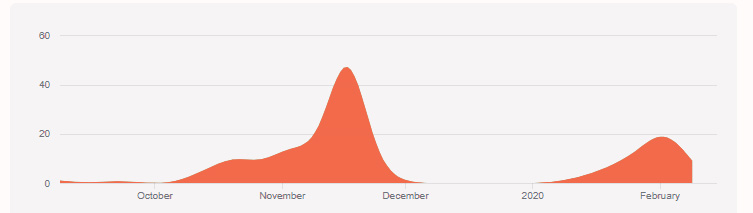
\includegraphics[width=\textwidth]{05Coding/05Pictures/contributions.jpg}
   \caption{Contributions to the Master branch (source: https://github.com/)}
\end{figure}

Nevertheless, this rigour in creating tickets was not always achievable. In particular, it was difficult to create sufficiently small tickets at the beginning of the development process when more fundamental components of the systems were being developed. In these cases, we assigned tickets to a pair or group of people. This approach achieved the following:

\begin{itemize}
    \item Improved the overall code quality and fastened production \cite{pairprogramming}.
    \item Minimised review time over the long run.
    \item Distributed the knowledge of large system components across a few people instead of one person.
    \item Eased introducing the new team member to the project.
\end{itemize}

In addition, we used a scrum board to get an overview of ongoing tickets. Although the Scrum community is engaged in an ongoing discussion about the benefits of a physical scrum board over an online one \cite{physicalscrum}, given we had no actual workplace, using the former was not possible. The board allowed us to see which tickets needed to be reviewed and which ones were ready to be merged. The tickets/cards were distributed into columns, such as `To do`, `In progress`, `Review in progress`, `Review complete` and `Finished`. A truncated picture of this scrum board can be seen on figure \figurename{\ref{Scrum}}.

\begin{figure}[H]
   \centering
   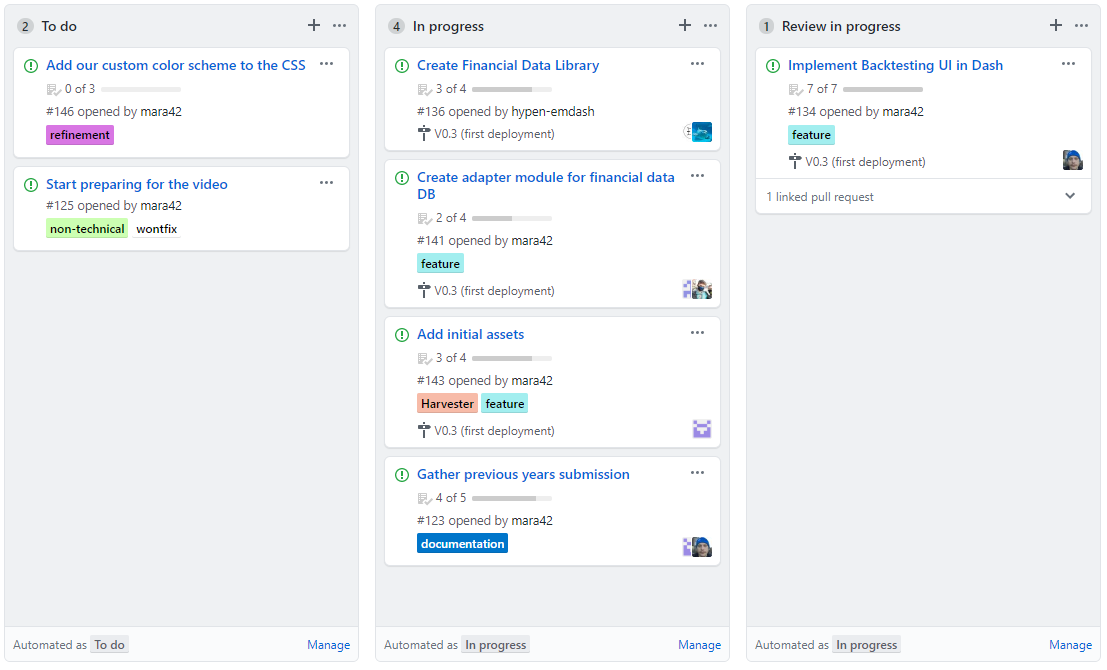
\includegraphics[width=\textwidth]{05Coding/05Pictures/scrumboard.png}
   \caption{Scrum board - truncated}
   \label{Scrum}
\end{figure}

The details of the workflow largely depended on the task at hand and the person working on it. The decision whether to do pair-programming or to work individually was left up to individual members. Before we commenced coding, the team agreed on a development environment and coding standards (for a detailed analysis, see \ref{Coding Standards}). Since this report was a relevant portion of the workload, we decided to treat it as code. The report was written in \LaTeX with an overall structure of the document defined in a main.tex file that linked to individual sections. This allowed members to work on different sections concurrently just as they could with the codebase.

%Isn't it the assignee that indicates its done and not the ticket creator?
Regardless of the nature of a ticket, the week, or in case of some larger tasks two week long cycle, ended with its creator indicating that the changes were ready to be integrated. This was done by publishing the changes and creating a new pull request, which - upon approval - pushed the changes onto the master branch of our project. To ensure code quality, we set up a continuous integration (CI) environment (more on that in \ref{Coding Standards}). After all checks passed, the changes were successfully integrated into the codebase.

\subsection{Key Implementation Decisions}

Let us now discuss the main technologies used in our project. These can be categorised as follows:

%%These next two are in really really well written but im not sure the tone is appropriate for a report. Its seems conversational at times. Ive tried my best to correct this, take it if you like it

\subsubsection{Web Framework}
\label{Web Framework}
Choosing the right web framework proved to be harder than we anticipated. The team identified the two major options available for Python to be Django and Flask. Although we decided to use Django for our first semester's minimum viable product (MVP), we had ended up spending a significant portion of our available time learning how to use it. At the beginning of the second semester, we had to decide whether we were would continue using Django or switch to Flask. In the end, we opted to go with Flask for the following reasons:

\begin{itemize}
    \item Django has one architecture that all projects must share, and we have designed the architecture for our project ourselves. While neither architecture is wrong, the two are not compatible. Flask, on the other hand, is structure-agnostic and therefore allows us to choose the layout of the code ourselves.

    \item Flask comes with the bare minimum features required for web-development, which means that we don't need to manage the complexity introduced by features we're not using. Django on the other hand comes prepackaged with a more complete feature-set. This would be desirable in a large web application, but introduces significant overhead in cases like ours, where our website has only a handful of pages.

%Maybe better just say SQL was a project requirement. The narrative should be finda was created as a reponse to a need / the requirement and not something we decided to do and the planned our web framework around
    \item Django all but insists on using its ORM for all database interaction. This conflicted with our plan to have a more manual approach through the use of the Finda module.
\end{itemize}

Thus, we chose Flask, a Python-based micro web framework. Flask provides the functionality required for building web applications, namely managing HTTP requests, using the `requests` library and rendering templates \cite{smyth_2018}. Flask leverages `Jinja2` as a template engine \cite{templates_2010}. We used the `render-template` library to process and parse HTML templates for all of our website's pages, except for the dashboard, which is described in more detail below. We used some of Flask's extensions, such as Flask-Login, which provides user session management\cite{flask-login} and `flask-wtf`, a wrapper for the `WTForms` package, to manage web forms \cite{wtforms-documentation}.

\subsubsection{GUI}
\label{GUI}

Dash is great for applications that require data visualisation, modelling, or analysis \cite{dash}, which is precisely what is needed for our portfolio backtesting software. It allows us to create reactive single-page apps, which means that with the use of tables, drop-down menus, and other forms of input, the app is updated instantly. This is done with the use of `callbacks` \cite{callbacks}. Callbacks allow us to exchange data with our web server asynchronously through AJAX requests whenever a user input changes. Upon receiving a response to such a request, the corresponding output is updated immediately without refreshing the page.

A typical callback using an example from our application can be seen below:

\begin{lstlisting}[language=Python, caption=setup.py - Development environment, label=lst:callback_example]
def register_add_portfolio_button(dashapp):
    dashapp.callback(
        Output("portfolios-container", "children"),
        [Input("add-portfolio-btn", "n_clicks")],
        [State("portfolios-container", "children")],
    )(add_portfolio)
\end{lstlisting}

% Isn't this too nitty-gritty? This is within a function level stuff

In this code snippet, we register a listener to the button with the unique id: `add-portfolio-btn`, and its property `n\_clicks`, or number of clicks. Whenever the input property changes, the corresponding function is called automatically. This also happens when the Dash page is first launched. Therefore, it is common to start the called function by catering to this case and raising a `PreventUpdate` exception if the input parameter is set to `None`. An example can be seen in \cite{prevent_update}.

The called function then receives the input properties as parameters. Furthermore, we can add any number of parameters as `State` objects as demonstrated above. When returning from a function call, the same number of values specified in the callback must also be returned. Mismatching the number of return values results in a runtime error. Mismatching the input parameters, on the other hand, yields a different function signature, and so the callback is not registered with the desired function. Doing this does not raise any errors.


%  Again, does how dev tool are accessed really need to be here? It stands out to me in the level of detail
Fortunately, Dash offers great developer tools \cite{dash_dev_tools}, such as the `Callback Graph` visible on \figurename{\ref{callback_graph}}, which can be accessed by running the application in debug mode and activating the Dev tools. This graph proved very useful, especially for the reasoning presented in \ref{dash_limitations}.

 \begin{figure}[H]
   \centering
   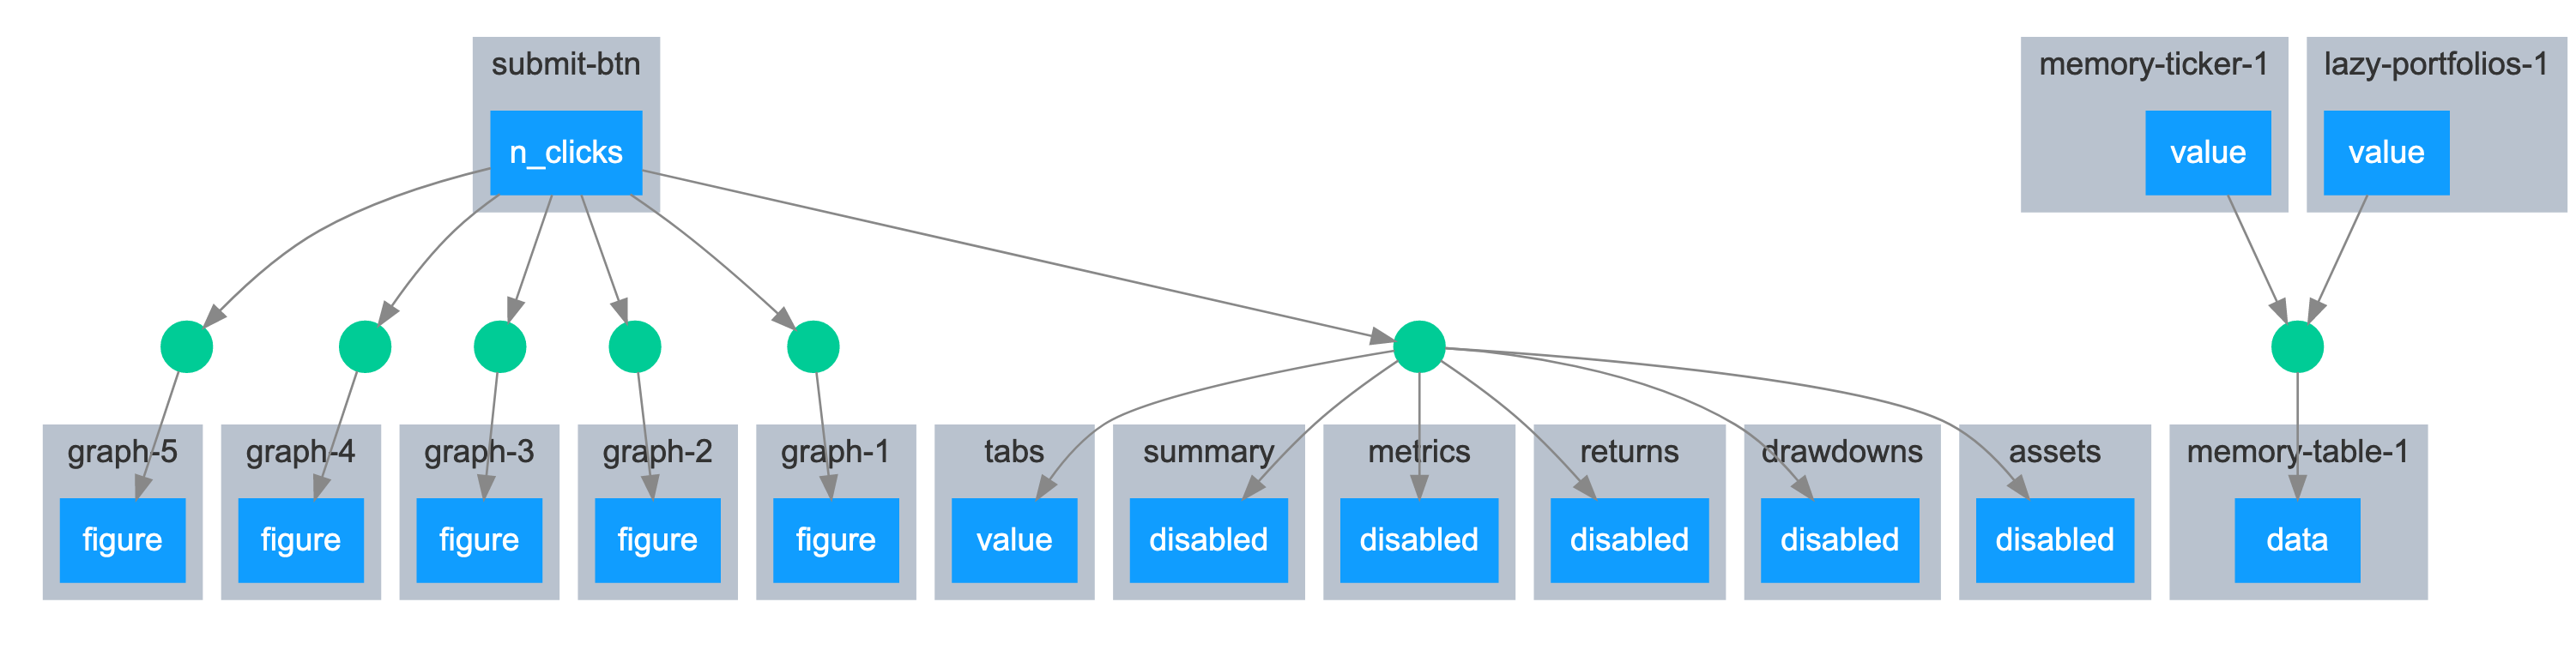
\includegraphics[width=\textwidth,keepaspectratio]{05Coding/05Pictures/callback_graph.png}
   \caption{Callback Graph on Thalia}
   \label{callback_graph}
\end{figure}


\subsubsection*{Limitations}
\label{dash_limitations}

Although Dash is fairly intuitive and well suited for one-page applications, it has its limitations when trying to dynamically create components. To be more precise, all callbacks need to be registered before runtime. In our application, the user is able to enter multiple portfolios via the `Add Portfolio` button. Doing so creates new input fields for the portfolio, which all need to be registered. 

As this problem persisted with other components as well, we were forced to try and find a general solution to this problem. Many approaches have been suggested by the Dash Community, some even by the development team \cite{dash_workaround}. In the end, we decided to use the most stable approach we identified, generating all components beforehand and hiding them from the user until activated. This means that the relevant function now also has the responsibility of returning the visibility of the required `div` element. Note that this is a highly requested feature in the Dash community, and is likely to be added soon, but for now, we are forced to resort to workarounds.

Furthermore, the data we show in the dashboard is centred around the strategy object discussed in \ref{BL Structure}. At the beginning of the backtesting process, a new strategy object is initialised, which is a time-costly task. As this object holds most of the information our result pages require, many functions would need to access the same object. 

One solution would be to have a callback for initialising the object, and then share it with all other methods. Although there exist ways to do so \cite{dash_share}, we were not satisfied with any of the approaches listed. Consequently, we decided to go forward with the original approach, which is also the approach favoured by Dash, and combine multiple outputs into one function. Although this introduced additional complexity to our code, it had a positive overall effect on the application's performance.

\subsubsection*{Layout}

The layout of the application, as discussed in \ref{GUI}, has been created with the use of the `Dash HTML components` library. Consequently, there was no need to write HTML for the dashboard, since the display elements were composed using Python. The library is then responsible for generating HTML content. Dash uses the Flask web framework, which makes it fairly simple to embed a Dash app at a specific route of an existing Flask app \cite{flask-dash}. The framework also handles most of the communications between the front-end and back-end.

The User-Interface was made with the use of `Bulma`, an open-source CSS framework \cite{bulma}. Bulma is ideal for creating responsive elements, as it automatically adapts the website to different screen sizes \cite{responsiveness_2020}. It is also compatible with most popular web browsers. Another advantage of Bulma is that we can create a very modern-looking website quickly since the framework automatically does a lot of work for us.

It also provides pre-styled elements, components (such as the navigation bar) and alerts for the users. Additionally, it is intuitive to learn when compared to `Bootstrap`, as Bulma uses memorable class names, such as `.button`, and has a very straightforward modifier system. It consists of nothing but CSS stylesheets without using any JavaScript and is therefore highly compatible with a framework like Dash.

\subsubsection{Business Logic}
\label{BL}

The business logic module sits at the very core of our application. We require it for producing a time series of a portfolio's performance as well as selected key risk metrics of a given asset allocation. This output is consumed by our web application and presented in plots and tables as described in \ref{GUI}.

Research into developing this module was initiated by listing our requirements for its desired behaviour. We identified that it should support:

\begin{itemize}
    \item Specification of a portfolio as a set of pandas Dataframes, the common data exchange format in our application.
    \item Calculation of a portfolio's return over time.
    \item Regular contributions to mimic saving.
    \item Rebalancing strategies to reestablish the desired weighting of a portfolio.
    \item Calculation of key metrics, including the Sharpe and Sortino Ratio, Max Drawdown, Best and Worst Year.
    \item Collecting and reinvesting dividends for equities.
\end{itemize}

Using these requirements, we struggled to find an open-source library that would handle these tasks for us. While backtesting libraries written in Python are available in abundance (e.g. PyAlgoTrade \cite{PyAlgoTrade} and bt \cite{bt}), each of these was found to be lacking in at least one critical aspect. None of them support specifying a portfolio using absolute or relative weights and instead seem to focus on backtesting trading strategies involving just a single asset while using technical indicators. Thus, we made the decision to develop our own library for handling the aforementioned tasks.

The result of this effort is `Anda`. For each of its functions, Anda takes as input a `Strategy` object that specifies the entire list of parameters needed to run a backtest, including contribution dates, a list of assets with associated price data, dividends for equities, etc. Calculations are performed on a per-metric basis by separating them into individual functions.
This approach has allowed us to tailor the entire business logic module to our specific needs and avoid having to produce complicated wrapper code for existing backtesting libraries.

\subsubsection{Database and Finda}
\label{Finda}

Another major technology decision was the choice of appropriate database management system (DBMS) for storing historical price data collected by the data harvester. Before committing to a specific technology, we identified the following requirements a suitable DBMS should fulfil:

\begin {itemize}
    \item \textbf{Schema:} The structure of our data is relatively simple. Consequently, Thalia does not require support for sophisticated features and data types. A suitable DBMS should be able to accommodate the database schema designed last term, with the addition of simple integrity constraints and cascade operations.
    \item \textbf{Support:} Ideally, the DBMS should be cross-platform, as this would allow us to defer commitment to a specific deployment platform until we are ready to start the CD process. 
    \item \textbf{License and pricing:} The DBMS should be free to use and have a non-restrictive license.
    \item \textbf{Performance:} The DBMS should be able to handle a high volume of concurrent reads to fulfil user requests. The data will be updated daily, meaning efficient write operations are a lower priority.
    \item \textbf{Usability:} As our team lacks experience in this field, a suitable DBMS should be relatively simple to learn. Ideally, team members should be able to learn the basics in a single week long sprint.
    \item \textbf{Security:} The DBMS should have a mature code base and be relatively secure, as access to financial data is a key component of our business model. Later, it will likely also store data that is not available through public APIs, meaning potential data breaches could expose us to legal liability. \cite{dataprotectionGov}
    \item \textbf{Type:} Since the project constraints specify we use SQL queries, only relational DBMSs supporting a version of SQL are appropriate.
\end{itemize}

MySQL, PostgreSQL, SQLite and MariaDB were subject to in-depth comparison based on fulfilment of the above requirements and industry adoption \cite{dbPerfComparison} \cite{dbmsMarketShare}. Our final decision was to use SQLite for the following reasons:
\begin{itemize}
    \item It is user-friendly and easy to deploy, allowing us to start continuous deployment faster.
    \item It has a small footprint and offers good performance \cite{dbPerfComparison}.
    \item Portable serverless design aids with development and testing.
    \item All team members have experience working with SQLite from previous term. This helps to reduce the overhead of knowledge transfer.
\end{itemize}

The main drawbacks of using SQLite, namely scalability and performance, are not a concern at this stage, as the current version of Thalia is meant to be a high-quality industrial prototype. As such, it will not contain the full range of financial data needed for marketability. Should SQLite prove to be inadequate in the future, we would be able to switch to a different DBMS with relatively little trouble, as the process of database migration is exceedingly well-documented \cite{frameworkDataMigration} \cite{understandingDataMigration}. To pre-empt any difficulties that might arise, the decision was made to design the data layer to easily accommodate such a migration.

% Ive switched up the subesctions here so there is one for each requirement. This way there is some structure to the DH section
% I also think a lot of this is more about design than technologies, so maybe this is the wrong section???!?!?!?!?!

\subsubsection{Data Harvester}
\label{Data Harvester}

The role of the Data Harvester is to collect live data from multiple sources, parse it to a format usable by the Anda library and store it with the Finda module. In addition to this, it contains a mechanism for managing collected data, so that our data collection can be adapted to user demands. Finally, it is responsible for making sure that all API requests made are compliant with the API's specified limitations, as breaching these could result in a ban and therefore haemorrhage data collection.

The following are the requirements our team identified for the Data Harvester module:

\begin{itemize}
    \item \textbf{Continuous Updating Mechanism:} The database has to be updated regularly to contain live data.
    \item \textbf{Redundancy:} As we are interfacing with third party software, redundancy measures must be implemented so that the Harvester can continue to gather live data in the event of an API call failing.
    \item \textbf{Maintenance:} Financial markets are dynamic and new financial instruments are constantly being created. Therefore, it must be easy for the team to add or remove assets from those tracked by the Harvester.
    \item \textbf{Standard Data Format:} To maintain data integrity and successfully interface with the Finda module, all data must be parsed to a standard format without sacrificing numerical accuracy or granularity.
    \item \textbf{Data Interpolation:} Some financial assets require interpolation to account for days on which data is unavailable (e.g. weekends and public holidays when most exchanges are closed).
    \item \textbf{Security:} Since the Data Harvester interfaces with external APIs, it must not introduce any significant vulnerabilities that may jeopardize Thalia's operation.
\end{itemize}

\subsubsection{Continuous Updating Mechanism and Maintenance}
This module of the Data Harvester was assigned the responsibility of regularly updating the database. It consists of a group of closely coupled components each fulfilling a specific role. These are:

\begin{itemize}
    \item \textbf{The run\_updates script} Running this script triggers a round of updates. It contains data for the specific configuration necessary to poll for each API (eg. the location of the API access key to be used and the number of calls to be made).
    \item \textbf{The update procedure} Runs a series of methods in turn. Firstly each supported API is checked for availability. For each asset assigned to that API, the module then fetches the appropriate amount of data. If the asset has no data available all data is collected from a fixed start date onwards. During this stage, the module also tracks the number of calls made to enforce compliance with the each API's terms and conditions. Whenever possible the Data Harvester makes sure that data is updated as soon as required so that the data stored is as close to being fully live as can be.
    \item \textbf{An initialiser} This sub-module loads and handles the persistent data specifying what assets and and asset classes to query APIs for. Persistent data is stored in CSV files so as to be human-readable. This makes it relatively easy to add support for new assets to the Harvester.
\end{itemize}

\begin{figure}[H]
    \centering
    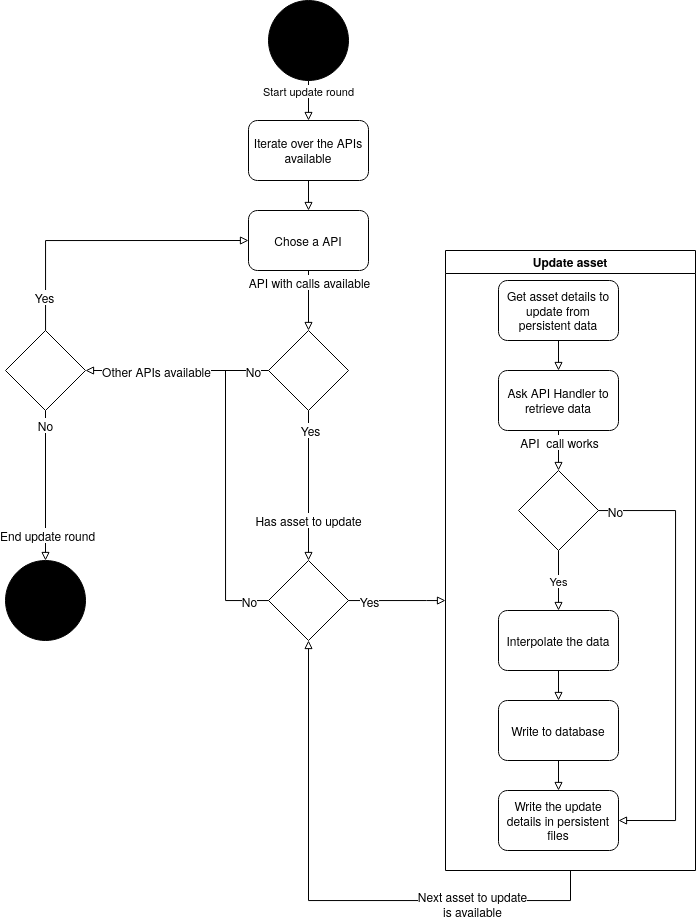
\includegraphics[width=0.7\textwidth]{04Design/04Pictures/update_mechanism_flow_chart.png}
    \caption{Flow chart for a round of updates\cite{TR}}
\end{figure}

For a more detailed breakdown of the updating mechanism refer to \ref{dhav_logs}.


\subsubsection{Redundancy}

Our current architecture allows for an asset to be served by several APIs. In the event of an API failure the asset's data can still be collected from another available source. This makes it simple to integrate a high degree of redundancy for popular assets into our product. 

% Dataframe format seems a bit too specific?

\subsubsection{Standard Data Format}
As previously discussed, all data written to the database is stored in pandas Dataframes. The Dataframes abide by the following format:

\begin{lstlisting}[language=Python, caption= Pandas Data Frame Format]
Columns: [AOpen<Decimal.decimal>, AClose<Decimal.decimal>,
          AHigh<Decimal.decimal>, ALow<Decimal.decimal>,
          IsInterpolated<Integer>] 
          
Index: [AssetTicker<String>, ADate <datetime.date>]
\end{lstlisting}

Data standardization is conducted as soon as the data has been received from the API. Each API is handled by a separate API Handler object. In addition to selecting what API to query for a specified asset this object ensures the data gathered has been converted to the appropriate format. The API Handler also logs any potential changes made to the data's format from the providers side.

\begin{figure}[H]
    \centering
    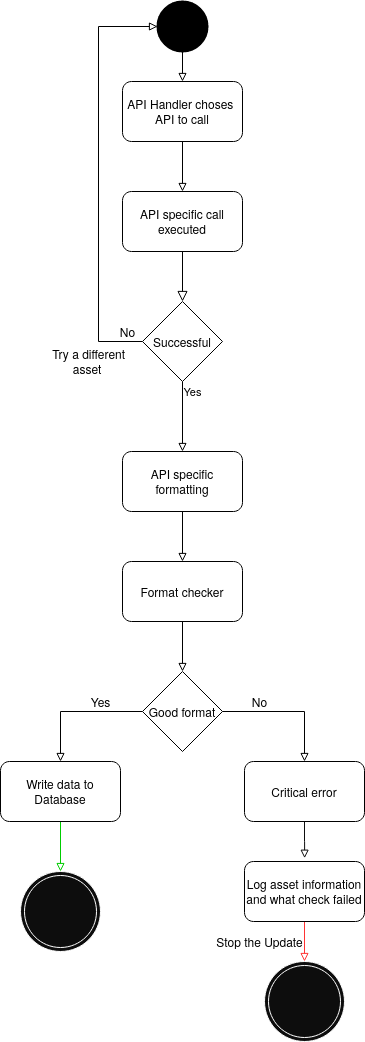
\includegraphics[width=0.47\textwidth]{04Design/04Pictures/api_handler_v3.png}
    \caption{API Handler Flow Chart \cite{TR}}
\end{figure}

\subsubsection{Data Interpolation}
The numerical analysis performed by the Anda library can only be sensibly run on continuous sets of data. Real world data is often messy and needs to be cleaned before it is suitable for further processing. In the case of asset prices, the form that this `messiness` manifests itself in are periods for which an asset isn't traded and therefore does not have a price. Additionally, data contained by APIs may not be complete and may therefore contain gaps for witch assets prices simply aren't recorded. The team decided to assign the responsibility of managing this uncertainty to the Data Harvester as it is loosely coupled to the other layers of our system. The Harvester manages such gaps through the process of nearest neighbour interpolation, where the last known price is assumed to hold for the entire duration of the gap. This practice is standard when considering financial data, and is how major exchanges report prices during weekends and bank holidays. Interpolated dates are flagged in the database to make sure this process is reversible. 

The following is a example of how such data is stored:
\textbf{\newline Pre-Interpolation: }
\begin{center}
    \begin{tabular}{||c c c c c c c c||} 
        \hline
        Index & ADate & AHigh & ALow & AOpen &A Close&AssetTicker&IsInterpolated\\ [0.5ex] 
        \hline\hline
        3&2000-11-16&126.86&126.89&126.86&87.36&VFIAX&0 \\ 
        \hline
        4&2000-11-17&126.44&126.44&126.44&87.07&VFIAX&0\\
        \hline
        5&2000-11-20&124.12&124.15&124.15&85.47&VFIAX&0\\ 
        \hline
        6&2000-11-21&124.55&124.45&124.55&85.78&VFIAX&0\\
        \hline
    \end{tabular}
\end{center}

\textbf{\newline Post-Interpolation: }
\begin{center}
    \begin{tabular}{||c c c c c c c c||} 
        \hline
        Index & ADate & AHigh & ALow & AOpen &A Close&AssetTicker&IsInterpolated\\ [0.5ex] 
        \hline\hline
        3&2000-11-16&126.86&126.89&126.86&87.36&VFIAX&0 \\ 
        \hline
        4&2000-11-17&126.44&126.44&126.44&87.07&VFIAX&0\\
        \hline
        5&2000-11-18&126.44&126.44&126.44&87.07&VFIAX&1
        \\
        \hline
        6&2000-11-19&126.44&126.44&126.44&87.07&VFIAX&1 \\
        \hline
        7&2000-11-20&124.12&124.15&124.15&85.47&VFIAX&0\\ 
        \hline
        8&2000-11-21&124.55&124.45&124.55&85.78&VFIAX&0\\
        \hline
    \end{tabular}
\end{center}

\subsubsection{Security}
In the future, we expect to collect data from sources that are not available free of charge. Additionally, our offering of financial data is key to our unique value proposition. It is therefore easy to see how a potential data breach could end up having catastrophic financial and legal implications for our company. To mitigate this risk, we decided to conduct an internal security audit of the Data Harvester module to identify any potential vulnerabilities. To do so, we created and analysed a scenario where an attacker is attempting to disrupt the operation or gain control of the Data Harvester. Our analysis yielded the following security concerns that needed to be preemptively addressed:

\newline
\textbf{Security Concerns}
\begin{enumerate}
    \item \textbf{API calls: }The data received from an API may be intercepted or modified.
    \item \textbf{API keys: }An attacker could gain control of API keys if not stored safely.
    \item \textbf{Rogue APIs: }An API can could send a malicious package instead of the expected data.
\end{enumerate}

We addressed these concerns in the following ways:

\textbf{Solutions}
\begin{enumerate}
    \item \textbf{API calls: }Depending on the API settings, we will use either an IPSec policy or a VPN connection. The details of this should first be discussed with the financial data provider.
    \item \textbf{API keys: }We will salt and then hash the API keys with SHA512 before storing them. Since the number of financial data APIs on the market is relatively small, we can use the SHA512 algorithm without worrying about computation time.
    \item \textbf{Rogue API: }We have added several checks to ensure data retrieved is what was expected. Should the Harvester receive malformed data, a critical error will be raised and the incident will be logged for later inspection. 
\end{enumerate}

\subsection{Integration and Deployment}
\label{Coding Standards}

%This is another section that is well written but strikes me as being worded too informally. Ive tried to 'boring' it up a bit, take it if you like it

Despite our focus on writing well documented, high quality code, the process of integrating our system's various components proved to be difficult. In the first term, the team spent a great deal of time on integration as many components of the system had difficulty working together. Since this term consisted of significantly more coding and less work on non-technical deliverables, we were able to significantly expand the suite of DevOps tools put in place to aid with this process \cite{DevOps}.

We decided to redesign the development environment from scratch instead of building directly on last term's. The list of libraries required by our project can be found in the `setup.py` file in the following lines of code:

\begin{lstlisting}[language=Python, caption=setup.py - Development environment, label=lst:Development_env]
"""A setuptools based setup module."""
from os import path

from setuptools import find_packages, setup

here = path.abspath(path.dirname(__file__))

install_requires = [
    "flask",
    "flask-login >= 0.5",
    "flask-migrate",
    "flask-wtf",
    "pandas",
    "dash",
]


tests_require = ["pytest", "coverage", ]

extras_require = {"dev": ["black", "flake8", "pre-commit"], "test": tests_require}

setup(
    name="Thalia",
    version="0.2.0",
    packages=find_packages(),
    install_requires=install_requires,
    extras_require=extras_require,
)
\end{lstlisting}

One of the first decisions we had to make was to choose a standard coding style. For this, we used `flake8`, which can be seen amongst the extras in the code snippet above. The original documentation of flake8 defines it as ``[...] a command-line utility for enforcing style consistency across Python projects. By default it includes lint checks provided by the PyFlakes project, PEP-0008 inspired style checks provided by the PyCodeStyle project, and McCabe complexity checking provided by the McCabe project`` \cite{flake8}. However, as is common practice, we also decided to redefine the maximum line-length as 88 instead of 79, as we found this convention to be a hindrance when writing code.

Another tool used to enforce uniform style was the `black` auto-formatter for Python \cite{black}, which formatted the code for us upon every save (if enabled) and when committing code to GitHub. This has been achieved by the use of githooks \cite{githooks}, which are programs that are triggered upon certain git actions. Setting up these hooks required the `pre-commit` package. This ensured that both flake8 and black were guaranteed to run before publishing changes.


\subsubsection{Continuous Integration}
\label{Continuous Integration}

Many studies have investigated the positive effects of developing in a continuous integration (CI) environment (see, for example, \cite{CI_1} and \cite{CI_2}). Regardless of the exact implementation, its obvious benefit is that it provides security and uniformity for projects. We already made some steps to achieve a uniform style but had no means to know whether the code published had also passed its tests. Note that, in this section, we will only discuss testing as a part of CI and not the testing strategy (for this, see \ref{Testing}).

Another important part of the DevOps toolchain is the use of containers, which is what Docker helps to achieve \cite{Docker}. Docker helps developers focus on writing code rather than worrying about the system the application will be running on and also helps to reveal dependency and library issues. As Docker is open source, there are many free to use docker images available online \cite{DockerImages}. When choosing the CI environment, Docker support was one of the main requirements.

The most promising candidate for this was CircleCI \cite{CircleCI}, which is a cloud-based system with first-class Docker support and a free trial. After connecting our GitHub repository to CircleCI and setting up a configuration, CircleCI now does the following on every pull-request:

\begin{enumerate}
    \item Sets up a clean Docker container or virtual machine for the code.
    \item Checks previously cached requirements (for more detail see \figurename{\ref{cache_CI}}).
    \item Installs the requirements from `requirements.txt`
    \item Caches the requirements for faster future performance.
    \item Clones the branch needed to be merged.
    \item Runs flake8 one last time and saves results.
    \item Runs tests and saves results.
    \item Deploys the master branch to AWS, see \ref{Continuous Deployment}
\end{enumerate}

 \begin{figure}[H]
   \centering
   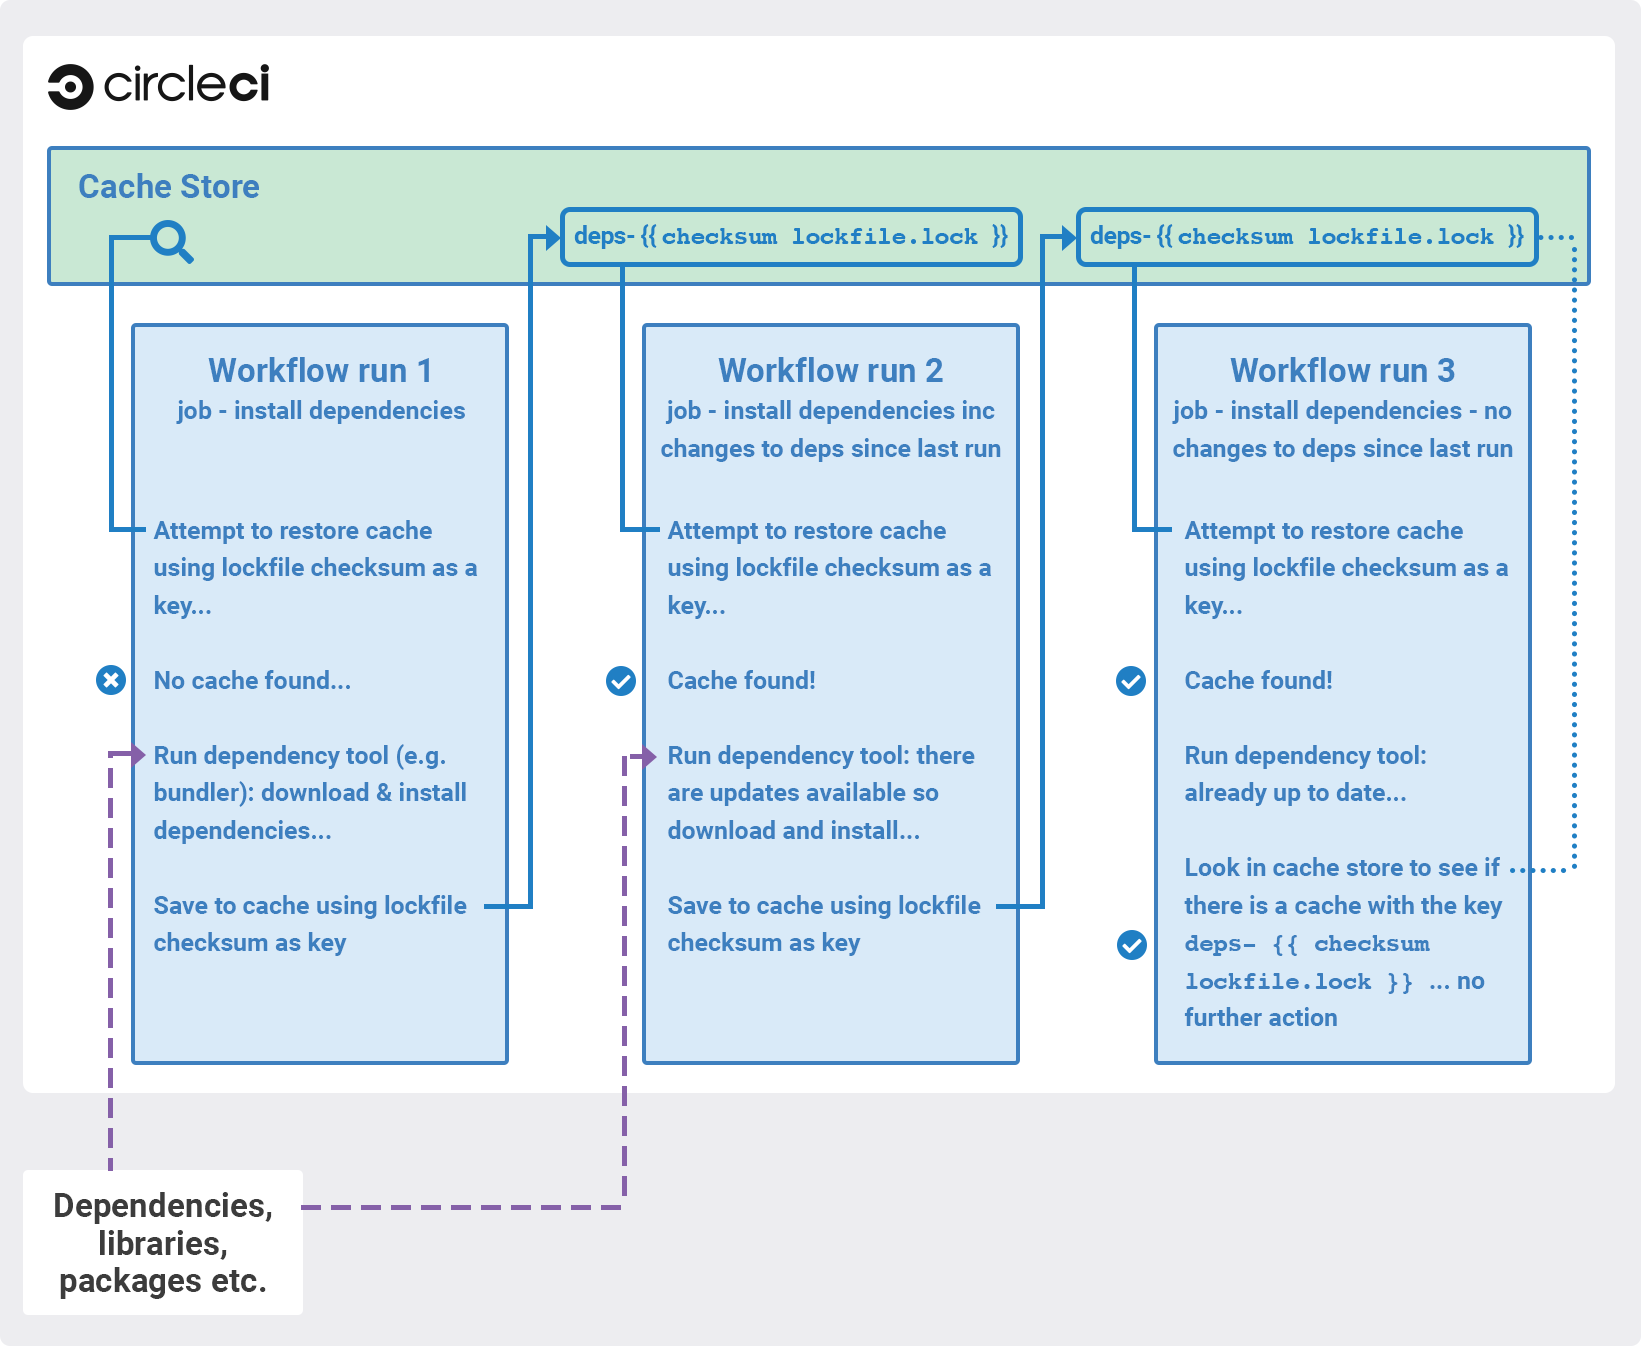
\includegraphics[width=\textwidth]{05Coding/05Pictures/cache_CI.png}
   \caption{CircleCI on Caching (source: https://circleci.com/docs/2.0/caching/)}
   \label{cache_CI}
\end{figure}

The outcome of these steps is visible on the CircleCI web platform, but - more importantly - also on GitHub. CircleCI will prevent a merge with master if failing tests (or no tests) have been found.

 \begin{figure}[H]
   \centering
   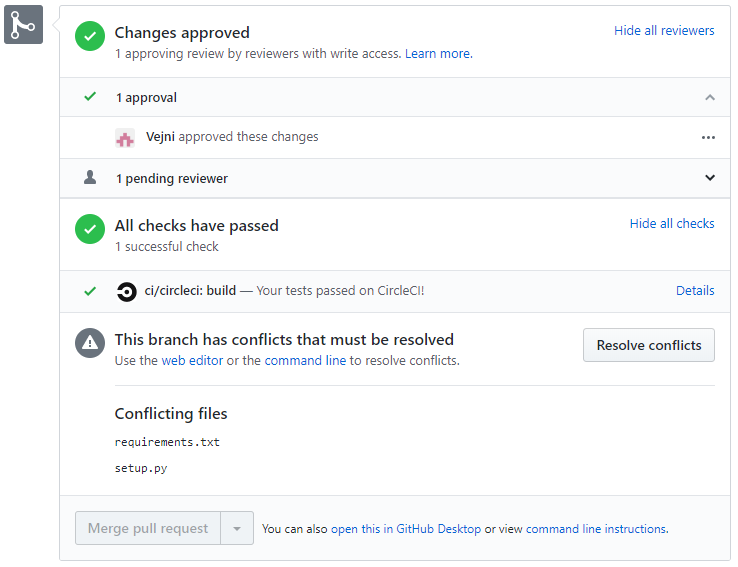
\includegraphics[scale=0.6]{05Coding/05Pictures/circleCI.png}
   \caption{CircleCI on GitHub (source: https://github.com/)}
   \label{CircleCI}
\end{figure}

With these steps, we managed to ensure that the code written is uniform and of good quality. It significantly reduced the time needed for integrating and code reviewing. The last step was now to deploy the system.

\subsubsection{Hosting and Continuous Deployment}
\label{Continuous Deployment}

An overview of the literature concerning deployment reveals a plethora of different strategies for deploying and hosting web applications \cite{ConnollyFundamentals}. Our decision of how to choose among them involved the following considerations:

\begin{itemize}
    \item Price - since our budget is severely constrained, we were looking for a cheap hosting solution
    \item CircleCI support - The target host should be supported by CircleCI natively to ease development of a continuous deployment (CD) pipeline
\end{itemize}

The upfront cost of buying physical servers ruled it out as an option for us. Thus, we turned our attention to solutions involving deployment to a virtual machine in the Cloud.

Due to native CircleCI support and a free-tier service, we initially chose Heroku \cite{Heroku} as our hosting provider. This allowed us to host our application for free in the nascent stages of development while providing ample opportunity for horizontal and vertical scaling later on if required.

However, it quickly became apparent that Heroku was not appropriate for our purposes, due to its lack of support for sqlite databases \cite{HerokuSqlite}. Hence, we moved to AWS \cite{AWS}, which is also supported by CircleCI \cite{AWSCircleCI}.

The benefits of using continuous deployment have been well established for multiple years and involve ``the ability to get faster feedback, the ability to deploy more often to keep customers satisfied, and improved quality and productivity`` \cite{CDBenefits}. Using AWS in combination with CircleCI, our CD pipeline involves the following simple steps:

\begin{enumerate}
    \item Upon commits to the master branch on GitHub, CircleCI triggers a workflow.
    \item The workflow first executes the steps listed in \ref{Continuous Integration} to ensure the validity of the current codebase state.
    \item If this step is successful, the master branch is pushed to a remote repository recognized by AWS via git.
    \item AWS executes the `Procfile` script stored in the root of our project to start the application using a `gunicorn` web server \cite{Gunicorn}.
\end{enumerate}

Our deployment process is thus fully automated and immune to failing tests, as it will only complete successfully if the application is in a correct state. The full CI/CD workflow is captured by the flowchart on \figurename{\ref{CI_CD}}.

 \begin{figure}[H]
   \centering
   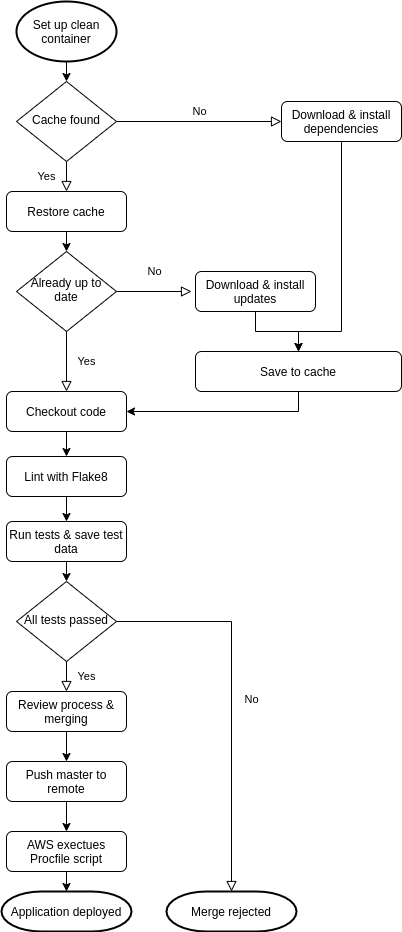
\includegraphics[scale=0.6]{05Coding/05Pictures/CI_CD.png}
   \caption{CI/CD workflow}
   \label{CI_CD}
\end{figure}

\end{document}
